Identifying likely failure modes is an important aspect of safe and secure operation of any large infrastructure. For a \ac{nrhes}, a large piece of infrastructure that has not yet been built, a design that addresses potential failures ensures long term safe, reliable, and profitable operation. This chapter will evaluate the economic, grid reliability, and physical risks of failures in the coupling of a \ac{npp} to an industrial process which functions in a dynamic fashion. Three preliminary hazard analyses will initially be applied to the safety, flexibility, and profitability of the system in order to do a cursory qualitative model of what concerns need to be taken into consideration. A fuzzy Analytic Hierarchy Process (f-AHP) will then be applied to various industrial process options to include in a model of a \ac{nrhes} thermally coupled to the \ac{npp}. The focus of this section is to develop a means of comparing various coupled industrial processes to determine which industrial process will be used in the exergy analysis.
\section{Risk Assessment Background}
Risk assessment is a means of analyzing complex systems for hazards. Often the risk assessment tools, such as probabilistic risk assessment, fault tree analysis, and failure mode and effects analysis, model many variables in large systems and attempt to contain them into an easy to understand table or number for comparison. Since there has yet to be a physical model of a \ac{nrhes} built, now is the appropriate time to assess risks in order to incorporate mitigating measures in the design basis. Incorporating risk management in the design of a facility minimizes the costs and dangers associated with the system in the long run.
%When determining an appropriate electricity generation source for a given region it is important to incorporate variables such as economic viability, emissions, flexibility, and reliability. A \ac{nrhes} is even more difficult to quantify as it supplies both electricity to the grid as well as a secondary product. The goal is to have a more economically robust system that emits less and is both more reliable and more flexible than any electricity generation source currently available.

\section{Preliminary Hazards Analysis}
As was done in Falcone et al. in establishing a new approach to risk assessment of cogeneration systems, this risk assessment will begin with a \ac{pha} \cite{Falcone}. The main purpose for a \ac{pha} is, as the name suggests, to identify hazards and possible implications of the design of a particular system or product.  A \ac{pha} is appropriate for the current state of development for a \ac{nrhes} due to it still being in the design stage. The goal of this \ac{pha} will be to highlight potential economic, reliability, and physical safety hazards. Performing a \ac{pha} at this early point in the life cycle of a \ac{nrhes} will hopefully reduce the resources spent on engineering design and potential construction errors. This analysis is not exhaustive but will address some of the more obvious concerns. The \ac{pha} will need to be updated as research continues and hazards are determined.
	Performing a \ac{pha} requires classifying the hazard level and frequency associated with each event. The hazard classes for this \ac{pha} range from Negligible to Catastrophic. A Class I hazard has negligible negative outcomes, a Class II hazard has marginal effects, a Class III hazard has critical impacts, and a Class IV hazard has catastrophic impacts \cite{ostrom2012risk}.  The frequency of occurrence estimates are qualitative as the values cannot be verified at this point. A discussion of Tables \ref{econ}, \ref{fluc}, and \ref{safety} is included in the following text.

\begin{landscape}
%\subsubsection{Economic PHA}
\begin{table}[h!]
\centering
\caption{Economic Preliminary Hazard Analysis}
\label{econ}
\begin{tabular}{|l|l|l|l|l|l|}
\hline
\textbf{\begin{tabular}[c]{@{}l@{}}Potential \\ Failure\end{tabular}} & \textbf{\begin{tabular}[c]{@{}l@{}}Event Causing\\ Hazardous\\ Condition\end{tabular}} & \textbf{\begin{tabular}[c]{@{}l@{}}Hazardous\\ Condition\end{tabular}}  & \textbf{Hazard Class} & \textbf{\begin{tabular}[c]{@{}l@{}}Preventative \\ Measure\end{tabular}} & \textbf{\begin{tabular}[c]{@{}l@{}}Qualitative\\ Likelihood\end{tabular}} \\
\hline
\begin{tabular}[c]{@{}l@{}}Industrial process\\ is not profitable \end{tabular}      & \begin{tabular}[c]{@{}l@{}}If the industrial\\ process has to be\\ ready to take load\\ from the grid, it \\ will likely be running\\ below capacity and \\ may not be profitable\end{tabular}      & \begin{tabular}[c]{@{}l@{}}Industrial \\ process loosing\\ money\end{tabular} & \begin{tabular}[c]{@{}l@{}}Class III:\\ the benefit of\\ the \ac{nrhes} \\ would be lost\\ without a means\\ of having the \\ industrial process\\ prepared to take \\ heat. \end{tabular}    & \begin{tabular}[c]{@{}l@{}}Contracts \\ ensuring\\ a certain profit\\ for the industrial\\ process to be \\ prepared to \\ take heat from\\ the Nuclear\\ Power Plant\end{tabular} & Likely \\
\hline
\begin{tabular}[c]{@{}l@{}}Nuclear regulations \\ could apply to the\\ whole system, \\ increasing the costs\\ of the system\end{tabular} & \begin{tabular}[c]{@{}l@{}}Since the \\ components will \\ be co-located \& \\ coupled, the NRC \\ may have\\ jurisdiction \\ over the whole system\end{tabular}  & \begin{tabular}[c]{@{}l@{}}Additional \\ regulations \\ on the industrial \\ process could \\ result in greater\\ costs\end{tabular} & \begin{tabular}[c]{@{}l@{}}Class III: without an \\ industrial process\\ the whole \ac{nrhes} \\ would be undermined.\end{tabular} & \begin{tabular}[c]{@{}l@{}}Determine regulatory \\ oversight before \\ beginning \\ construction\end{tabular} & \begin{tabular}[c]{@{}l@{}}Fairly Likely\\ as the other\\ components\\ would be\\ within the\\ required \\ boundary \\ around the NPP\end{tabular} \\
\hline
\begin{tabular}[c]{@{}l@{}}Feedstock\\ Costs Rising \end{tabular} & \begin{tabular}[c]{@{}l@{}}Any of the feedstocks\\  could rise in price for \\ any number of reasons. \\ Rise in price during \\ the operation of the \\ system could result in \\ the product prices no \\ longer being\\ competitive\end{tabular} & \begin{tabular}[c]{@{}l@{}}Feedstocks rising in \\ price during the \\ operation of the system \\ could\\ result in the \\ product prices no \\ longer being \\ competitive\end{tabular} & \begin{tabular}[c]{@{}l@{}}Class I: shifts \\ already occur in\\ feed stock prices and\\ are systems adjust.\end{tabular}  & \begin{tabular}[c]{@{}l@{}}Include long term \\ projections for the \\ feedstock costs of \\ the various \\ components in the \\ design phase of the \\ \ac{nrhes}\end{tabular}                      & \begin{tabular}[c]{@{}l@{}}Likely there \\ will be \\ fluctuations.\\ Depends on the \\ feedstock\end{tabular}\\
\hline
\begin{tabular}[c]{@{}l@{}}Product Value\\Decreasing\end{tabular} & \begin{tabular}[c]{@{}l@{}}There could be a \\ change in \\ conditions or a \\ new technology \\ that makes the \\ industrial process \\ product value \\ decrease\end{tabular} & \begin{tabular}[c]{@{}l@{}}For each of the products,\\ the reason would be \\ different. Desal: a \\ drought could end\\ Syn fuel: oil prices \\ could decrease\\ Hydrogen: Less \\ energy\\ intensive \\ process could be \\ invented\end{tabular} & \begin{tabular}[c]{@{}l@{}}Class II: the industrial \\ process would need\\ to be further subsidized\\ by other components \\ to continue to run\end{tabular}& \begin{tabular}[c]{@{}l@{}}Do long term \\ economic \\ analysis of the \\ industrial \\ process. Pick \\ a product \\ or location where\\ the product will \\ clearly be in demand\end{tabular} & \begin{tabular}[c]{@{}l@{}}Possible: The \\ product value \\ will likely \\ fluctuate over \\ the length of \\ the\\ project\end{tabular}          \\ \hline
\end{tabular}
\label{economic}
\end{table}                                           \end{landscape}



\begin{landscape}
%\subsection{Grid Reliability PHA}
\begin{table}[h!]
\centering
\caption{Grid Reliability Preliminary Hazard Analysis}
\label{fluc}
\begin{tabular}{|l|l|l|l|l|l|}
\hline
\textbf{\begin{tabular}[c]{@{}l@{}}Potential \\ Failure\end{tabular}} & \textbf{\begin{tabular}[c]{@{}l@{}}Event Causing\\ Hazardous\\ Condition\end{tabular}} & \textbf{\begin{tabular}[c]{@{}l@{}}Hazardous\\ Condition\end{tabular}} & \textbf{Hazard Class} & \textbf{\begin{tabular}[c]{@{}l@{}}Preventative \\ Measure\end{tabular}}  & \textbf{\begin{tabular}[c]{@{}l@{}}Qualitative\\ Likelihood\end{tabular}} \\
\hline
\begin{tabular}[c]{@{}l@{}}Nuclear Power \\ Plant Outage\end{tabular}  & \begin{tabular}[c]{@{}l@{}}The NPP needs \\ to be refueled\end{tabular} & \begin{tabular}[c]{@{}l@{}}NPP down for \\ refueling\end{tabular} & \begin{tabular}[c]{@{}l@{}}Class I: This will \\ be a routine issue. \\ The industrial \\ process will need \\ to stop during the \\ outage and the \\ grid will need to \\ get electricity \\ from peaker\\ plants\end{tabular} & \begin{tabular}[c]{@{}l@{}}Plan ahead with the \\ industrial process \\ so that it can either \\ get\\ electricity from\\ the grid or be \\ paid to close for \\ the outage.\end{tabular}                                     & \begin{tabular}[c]{@{}l@{}}Certain: an \\ NPP needs to \\ be refueled\end{tabular} \\
\hline
\begin{tabular}[c]{@{}l@{}}System not able \\ to quickly shift\\  heat from \\ industrial process \\ to\\ electricity \\ generation\end{tabular} & \begin{tabular}[c]{@{}l@{}}The NPP heat \\ transport system \\ taking a while to \\ shift.\end{tabular} & \begin{tabular}[c]{@{}l@{}}The \ac{nrhes} is \\ briefly unable \\ to meet \\ the grid demand\end{tabular} & \begin{tabular}[c]{@{}l@{}}Class II: There \\ would be some \\ money loss as \\ some other \\ electricity \\ generation system \\ would supply the \\ demanded energy \\ during the transition \\ period\end{tabular}            & \begin{tabular}[c]{@{}l@{}}Include the time it \\ takes to allocate \\ heat in models of \\ the \ac{nrhes} to \\ determine how \\ much of a limiting \\ factor it is likely to be.\\ Include a battery in\\ the \ac{nrhes}\end{tabular} & Likely \\                       \hline
\end{tabular}
\label{fluctuate}
\end{table}
\end{landscape}



\begin{landscape}
%\subsection{Physical PHA}
\begin{table}[h!]
\centering
\caption{Physical Preliminary Hazards Analysis}
\label{safety}
\begin{tabular}{|l|l|l|l|l|l|}
\hline
\textbf{\begin{tabular}[c]{@{}l@{}}Potential \\ Failure\end{tabular}}                        & \textbf{\begin{tabular}[c]{@{}l@{}}Event Causing\\ Hazardous\\ Condition\end{tabular}} & \textbf{\begin{tabular}[c]{@{}l@{}}Hazardous\\ Condition\end{tabular}} & \textbf{Hazard Class} & \textbf{\begin{tabular}[c]{@{}l@{}}Preventative \\ Measure\end{tabular}} & \textbf{\begin{tabular}[c]{@{}l@{}}Qualitative\\ Likelihood\end{tabular}}                 \\
\hline
\begin{tabular}[c]{@{}l@{}}Materials failure \\ in the heat \\ transport system\end{tabular} & \begin{tabular}[c]{@{}l@{}}\ac{nrhess} are very \\ dynamic systems. \\ There will likely \\ be greater materials \\ wear due to the \\ dynamisticity of \\ the system\end{tabular} & \begin{tabular}[c]{@{}l@{}}Heat transport \\ pipe forms a leak\end{tabular}            & \begin{tabular}[c]{@{}l@{}}Class III:There \\ would be a loss \\ of\\ money due \\ to the shutdown \\ of the system\end{tabular}                                                                                                          & \begin{tabular}[c]{@{}l@{}}Reliable maintenance \\ \& appropriate choice \\ of heat transport \\ system\\ materials\end{tabular} & Possible                                                                                  \\
\hline
Release of Radionuclides                                                                     & \begin{tabular}[c]{@{}l@{}}Radionuclides \\ would need to \\ escape first into \\ the heat transport \\ system and then from \\ the heat transport system \\to the environment\end{tabular}                                                                                          & \begin{tabular}[c]{@{}l@{}}A large release \\ of airborne\\ radionuclides\end{tabular} & \begin{tabular}[c]{@{}l@{}}Class IV: A \\ radiation release \\ that could \\ potentially impact \\ human health \\ would have\\ massive negative \\ impacts for the \\ nuclear industry \& \\ would shut down \\ the\\ \ac{nrhes}\end{tabular} & \begin{tabular}[c]{@{}l@{}}Passive safety \\ systems, excellent \\ safety culture, \\ good reactor design\end{tabular}           & \begin{tabular}[c]{@{}l@{}}Unlikely: Based \\ on history of \\ NPP operation\end{tabular} \\
\hline
\end{tabular}
\end{table}
\end{landscape}

The initial economic \ac{pha}, Table \ref{econ}, demonstrates the importance of having detailed agreements between the various members of a \ac{nrhes} industrial park before construction begins.  Likely, the whole system would function better under a single owner.  A single owner could allow an aspect of the \ac{nrhes}, such as the industrial process, to loose money and still be economic overall. Further avenues which need to be investigated before the construction of an industrial park include understanding the regulatory impacts and the long term projected worth of the products generated.

The initial grid reliability \ac{pha}, Table \ref{fluc}, demonstrates the importance of understanding how coupling an NPP to an industrial process will require a change of the scheduling approach to a nuclear power plant. Nuclear power plants require immense amounts of planning and scheduling in order to ensure safe operation of the plant.  Increasing the complexity by coupling the nuclear power plant to other systems will increase the complexity of scheduling activities such as outages as well as optimizing the heat and electricity output of the system to match the grid demand.

The initial physical \ac{pha}, Table \ref{safety},  demonstrates how, if done correctly, a thermally coupled industrial process to a nuclear power plant does not have to decrease the operational safety of the system.  Since nuclear power plants already have a lot of techniques in place to ensure a safe system that will not harm the public or the environment, those same approaches should be applied to the thermally coupled system. The existing infrastructure, including the safety culture, could be extended to the thermal coupling. Thermal coupling is used throughout this thesis as the use of heat from the \ac{npp} to directly support an industrial process.  Electrical coupling, for comparison, takes the electricity generated by the \ac{npp} which is then used to do electrical work or converted into heat or mechanical work to produce the desired product in the industrial process.


\section{Analytic Hierarchy Process}
The fuzzy \ac{ahp} developed and applied in this research compares \ac{nrhess} that include thermal coupling to three types of industrial processes: desalination, synthetic fuel production, and hydrogen production.  The AHP evaluates the profitability, flexibility, and safety characteristics in the coupling of a nuclear power plant to each of the given industrial processes. While AHP has been applied to energy systems in the literature, the application to a \ac{nrhess} is novel. An AHP approach provides important information into design considerations and quantitatively approaches, through expert opinion, which alternative is likely to be strongest given the criteria chosen. As \ac{nrhess} are currently in the research and development stage, AHP is a beneficial tool to develop for future decision making for \ac{nrhess}s.

An AHP uses pairwise comparisons of various potential options depending on a set of predetermined characteristics. Originally developed in the 1970s by Thomas L. Saaty, AHP has been applied to everything from determining appropriate bridge construction \cite{Pan2008}, to the appropriate energy generation mix in Turkey \cite{Kahraman2010, Saaty1987}. AHP is a multicriteria decision-making tool. There is a wealth of research applying multicriteria decision-making tools to energy planning. Pohekar et al. reviewed more than 90 published papers on multi-criteria decision making and energy planning and found \ac{ahp} to be the most popular \cite{Pohekar2004}. The reasons for the prevalence of AHP in energy planning, Pohekar et al. suggests, is due to its ability to:
\begin{quote}
	"convert a complex problem into a simple hierarchy, flexibility, intuitive appeal, its ability to mix qualitative as well as quantitative criteria in the same decision framework and use of computational aids leading to successful decisions in many domains.\cite{Pohekar2004}"
 \end{quote}
Some of the previous applications of AHP to energy systems noted in Pohekar et al. include Akash et al.  1999; and Ramanathan et al. 1995. Akash et al. uses AHP to analyze the selection of power plants in Jordan \cite{Akash1999}.  Ramanathan et al. applies AHP at a household level in India to determine which energy resources work best for various tasks in the home such as heating, water pumping, lighting, and household appliances \cite{Ramanathan1995}.

The general process for applying AHP involves initially determining a set of alternatives and a set of criteria on which to compare the alternatives. The hierarchy comes from the objective being structured above the criteria, which is then structured above the alternatives, as can be seen in figure \ref{AHP_struct}. To find the relative value of one of the alternatives over the other, the AHP approach develops a series of pairwise comparisons creating a ratio scale.  Generally AHP is performed on a scale of one to nine. After creating the ratio scale, the AHP approach applies an eigenvalue method to include the relative weights of each of the criteria to each of  the elements. Finally, the relative weights are combined with the ratios forming one measurement to compare the various elements.

\begin{figure}[h!]
  \centering
  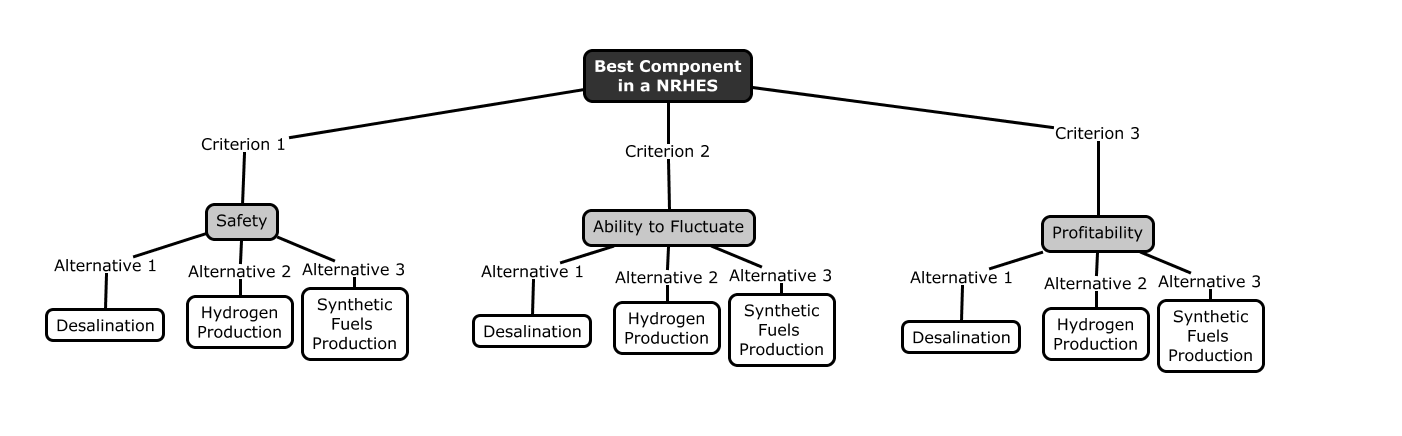
\includegraphics[width=0.9\textwidth]{AHP_hierarchy.PNG}
  \caption{\small \sl The overall hierarchy of the industrial processes under evaluation for inclusion in the \ac{nrhes}}
  \label{AHP_struct}
\end{figure}

The AHP not only provides insight into which is the best overall choice given the inputs and weights, but also which is the strongest candidate for each of the criterion. During the AHP process, before aggregating the values into one measurement, there are clear measurements of each of the alternatives in each of the criterion. The subjective nature of expert judgment as data requires a means of evaluation. As a check on the validity of the data, a traditional AHP measures the consistency of the values given by the experts using a Consistency Ratio, which needs to be less than 0.1, or 10\%, in order to be considered consistent. The Consistency Ratio compares the randomness of the expert judgments to a Random Consistency Index \cite{Saaty1987}.  If the consistency ratio is greater than 0.1, the data is judged to be too close to random.


\section{Fuzzy AHP}
Fuzzy logic applied to AHP takes into consideration the uncertainty inherent in a small number of expert opinions. Fuzzy AHP is an extension of the original AHP developed by Saaty in the 1970s \cite{Saaty1987}. Since Saaty's original development of AHP, multiple means of fuzzy AHP have emerged. Some notable fuzzy AHP approaches, as noted in \cite{Kahraman2010} include:
\begin{itemize}
\item Van Laarhoven and Pedrycz's approach from 1983 using triangular membership functions
\item Buckley's 1985 use of trapezoidal membership functions to determine fuzzy priorities
\item Cheng's 1997 approach focused on the grade value of the membership function.
\item Kahraman et al. generated a fuzzy weighted evaluation \cite{Kahraman2010}
\item Chang presented a new approach first determining triangular fuzzy numbers, then applying extent analysis method \cite{Chang1996}
\end{itemize}

 In the Buckley approach to fuzzy AHP, which is applied in this paper, $\alpha$ represents a value between zero and one reflecting the uncertainty.  Uncertainty is greatest when $\alpha$ is close to zero and least when close to one. As can be seen in figure \ref{fuzzy_exp}, in a trapezoidal membership approach, the lower left point of the triangle, where $\alpha$ equals zero, is the minimum fuzzy number, the points making up the middle represent the most likely fuzzy number, and the point at a y value of zero on the right represents the maximum fuzzy number \cite{Pan2008}. The higher the fuzzy number on the x axis, the more important that criteria is, or the stronger the alternative.
\begin{figure}[h!]
  \centering
  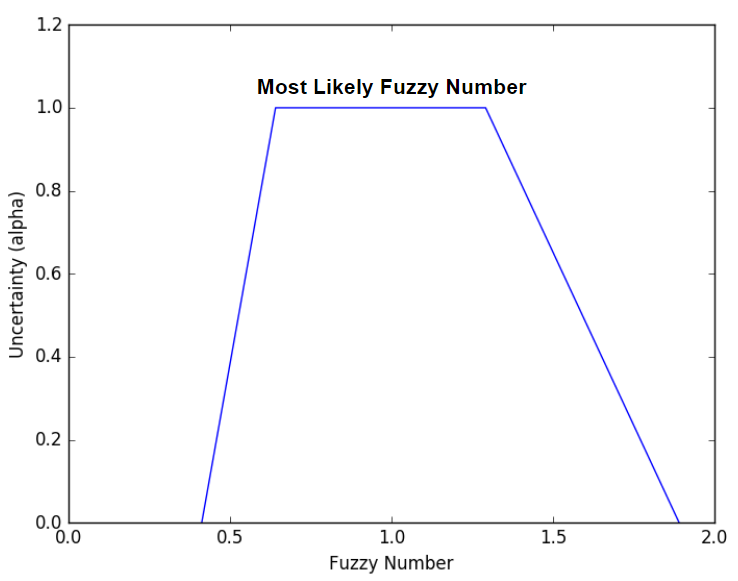
\includegraphics[width=0.5\textwidth]{fuzzy_explaination.png}
   \caption{\small \sl Representation of the meaning behind the membership function graph for the fuzzy numbers}
   \label{fuzzy_exp}
\end{figure}

 As described in \cite{Kahraman2010}, after receiving the numbers from the decision makers, the fuzzy weight can be found by determining the geometric mean for each row in each of the AHP matrices:

 \begin{equation}
 z_i=[\prod_{j=1}^n t_{ij}]^{\frac{1}{n}},
 \end{equation} where $t_{ij}=(a_{ij},b_{ij}, c_{ij}, d_{ij})$ correspond to the fuzzy values in Table \ref{fuzzyfit}. $n$ is the number of values in each row.  For example, if three experts were taking a survey with three pairwise comparisons, there would be nine total answers in each row. To find the performance scores ($r$), first sum each of the geometric means in each row, then weight each of the values accordingly:

\begin{equation}
r_{ij}=(\frac{a_i}{d},\frac{b_i}{c},\frac{c_i}{b},\frac{d_i}{a})
\end{equation}

To find the fuzzy utility:

\begin{equation}
U_i=\sum_{j=1}^n w_j*r_{ij},
\end{equation} where w is the weight found by the comparison of the importance of the various criteria to one another. To find the membership function $M(x)$, take the lowest value of the utility set and set the membership function to zero.  For the middle values of the utility set, the membership function is one. For all values greater than the greatest member of the utility set, the membership function is zero. For a utility set $(x_1,x_2,x_3,x_4)$

\begin{center}
\begin{table}
\centering
 \caption{The different x values correspond to the values on the y axis of the graph shown in figure 2.2.  When the likelihood of a certain fuzzy number being correct is very low, the y value is zero.  When it is more likely, the y value is one.}
\begin{tabular}{ |c|c| }
 \hline
 x & M(x)\\
 \hline
 $\leq x_1$  & 0 \\
 $\geq x_4$ & 0  \\
 $x_2 \leq x \leq x_3$ & 1  \\
 $x_1 \leq x \leq x_2$ & $\alpha \in [0,1]$\\
 $x_3 \leq x \leq x_4$ & $\alpha \in [0,1]$\\
 \hline
\end{tabular}
 \label{fuzzyfit}
\end{table}
\end{center}

\begin{table}[h!]
\centering
\caption{Fuzzy Logic Value Mapping}
\label{Fuzzy values}
\begin{tabular}{|l|l|l|}
\hline
\textbf{Description }                                                           & \textbf{Values }       & \textbf{Inverse}           \\
\hline
Equal                                                                  & (1, 1, 1, 1)     & (1, 1, 1, 1)         \\
\hline
Equal Importance                                                       & (1/2, 3/4, 5/4, 3/2) & (2/3, 4/5, 4/3, 2)      \\
\hline
Weak Importance                                                        & (1, 3/2, 5/2, 3)   & (1/3, 2/5, 2/3, 1)   \\
\hline
Strong Importance                                                      & (2, 5/2, 7/2, 4)     & (1/4, 2/7, 2/5, 1/2) \\
\hline
\begin{tabular}[c]{@{}l@{}}Very Strong\\ Importance\end{tabular}       & (5, 11/2, 13/2, 7)     & (1/7, 2/11, 2/13, 1/5) \\\hline
\begin{tabular}[c]{@{}l@{}}Absolutely Strong\\ Importance\end{tabular} & (7, 15/2, 17/2, 9)     & (1/9, 2/17, 2/15, 1/7)\\
\hline
\end{tabular}
\end{table}

\section{Expert AHP Survey}
The objective for the expert AHP survey is to determine the optimal industrial process to include in a generic \ac{nrhes} industrial park based on three criteria. The industrial process options are desalination, high temperature steam electrolysis for hydrogen production, and synthetic fuel production. The criteria the options are judged on are flexibility, safety, and profitability. The optimal way to perform an Analytic Hierarchy Process (AHP) is to gather a group of experts with complementary specializations in a general field to discuss the relative values of various options under determined criteria. For example, performing an AHP to determine the optimal industrial process in a \ac{nrhes} would best be done by gathering a group of experts in \ac{nrhess}s with specialties in understanding each of the specific industrial processes. The group could discuss the relative values to give to each of the alternatives for a given criterion. Due to the struggles of getting a group of \ac{nrhes} experts together in the same place, the values found for this research came from sending a survey to experts.  Other AHP evaluations employ similar methods\cite{Pan2008}. For this research, an expert is defined as someone who has published research or reports on \ac{nrhess}.

	The alternatives of desalination, hydrogen production, and synthetic fuels production were chosen due to their prominent role in research surrounding \ac{nrhess} \cite{Bragg-Sitton2014,Locatelli2015,Kim2016,Bragg-Sitton2016,Garcia2016,Shropshire2011, Ruth2014,Bienvenu2015}.  The criterion of flexibility was chosen as the industrial process in a \ac{nrhes} will need to be able to fluctuate to adjust to change demand as well as the dynamic generation from the industrial process.  The criterion of safety was chosen due to the inherent need for safety, especially within the context of the nuclear safety culture.  Safety underlies both the characteristic of flexibility and profitability. If the industrial process is not safe, it will not run, and therefore the other two characteristics are negligible. Profitability was chosen due to the whole \ac{nrhes} needing to be profitable in order to continue to run.  The industrial process provides a secondary source of income  increasing the overall profitability of the system as a whole.

There were five experts who completed the Analytic Hierarchy Process for a Nuclear Renewable Hybrid Energy System survey. Due to the small number of experts included in the survey, a fuzzy systems approach has been applied to the AHP. Tsyganok et al. determined that the expert competence should always be taken into consideration, especially when there are less than 50 experts included in the evaluation \cite{Tsyganok2012}. Thus, in this case, a fuzzy approach is clearly applicable due to the low number of responses.

 For this research, the same \ac{nrhes} with only the industrial process switched out will be compared. The assumptions for this research include:
\begin{itemize}
\item The process used for hydrogen production is high temperature steam electrolysis with thermal as well as electrical coupling to the nuclear power plant.
\item  The process for desalination is thermal desalination through distillation directly using heat from the nuclear power plant.
\item The synthetic fuel process is a Fischer-Tropsch method using coal as the hydrocarbon source.
\item Each of the processes consumes the same amount of heat from the nuclear power plant. While this would almost certainly not be true, it does make profitability comparisons easier.
\item All of the industrial processes are thermally coupled
\item Regional accessibility of feedstocks for each of the industrial processes are the same
\item Regional transportation costs are the same
\item Regulatory and taxation costs are the same
\end{itemize}

As can be seen in Table \ref{scale}, the scale for the answers for the second part of the question, Q1b and Q2b, ranged from two to  nine.  In the initial question the expert determines which of the alternatives better fits the criteria.  If the two alternatives were judged to equally answer the question, then a value of 1 was assigned to the relative importance of both. Table \ref{scale} displays the relative values for each of the characteristics considered in the AHP. The values are chosen on a scale of one to nine, with the industrial process strongly reflecting that characteristic receiving a nine and the characteristic relatively less reflecting those characteristics receiving appropriate smaller numbers. While the safety of the system is in reality the most important characteristic, as it is the foundation which the economic and grid reliability characteristics rely on, the safety issues are the easiest to mitigate and the most well known.

\begin{table}[h!]
\centering
\caption{Example of questions given in the Expert AHP survey}
\label{AHPQuestions}
\begin{tabular}{l}
Questions included in the expert AHP survey:                                                                                   \\ \hline
\multicolumn{1}{|l|}{\begin{tabular}[c]{@{}l@{}}Q1a: Do you think that the flexibility,is more important\\ than profitability of an industrial process?\\ Q1b: From 2 to 9, how would you compare the importance of \\ safety of an industrial process to the ability of the industrial process to fluctuate?\\ Q2a: Do you think that the flexibility,is more important than \\ profitability of an industrial process?\\ Q2b: From 2 to 9, how would would you compare the importance \\ of safety of an industrial process to the ability of the industrial process to fluctuate?\end{tabular}} \\ \hline
\end{tabular}
\label{questions}
\end{table}

\begin{table}[h!]
\centering
\caption{AHP Scale Description}
\label{AHPScale}
\begin{tabular}{|l|l|l|}
\hline
Quantitative Value & Explanation                                                                                                                              & Verbal Judgement                                                        \\ \hline
1                  & \begin{tabular}[c]{@{}l@{}}They are equally important \\ or equally meet the criterion\end{tabular}                                      & Equally more important                                                  \\ \hline
2                  & \begin{tabular}[c]{@{}l@{}}Experience and judgement \\ favor one alternative over \\ the other by a small margin\end{tabular}            & Weakly more important                                                   \\ \hline
3                  & \begin{tabular}[c]{@{}l@{}}Experience and judgement \\ moderately favor one \\ alternative over the other\end{tabular}                   & Weakly more important                                                   \\ \hline
4                  & \begin{tabular}[c]{@{}l@{}}Experience and judgement \\ clearly favor one \\ alternative over the other\end{tabular}                      & Strongly more important                                                 \\ \hline
5                  & \begin{tabular}[c]{@{}l@{}}Experience and judgement \\ strongly favor one \\ alternative over the other\end{tabular}                     & Strongly more important                                                 \\ \hline
6                  & \begin{tabular}[c]{@{}l@{}}Practice suggests moderate\\ preference for one alternative \\ over the other\end{tabular}                    & \begin{tabular}[c]{@{}l@{}}Very strongly more\\ important\end{tabular}  \\ \hline
7                  & \begin{tabular}[c]{@{}l@{}}One alternative is favored \\ very strongly over the other \\ and has been shown in practice\end{tabular}     & \begin{tabular}[c]{@{}l@{}}Very strongly more \\ important\end{tabular} \\ \hline
8                  & \begin{tabular}[c]{@{}l@{}}It is fairly clear that, in practice\\ one alternative is better than the \\ other\end{tabular}               & \begin{tabular}[c]{@{}l@{}}Absolutely more \\ important\end{tabular}    \\ \hline
9                  & \begin{tabular}[c]{@{}l@{}}The evidence favoring one \\ alternative over the other is of\\ the highest possible affirmation\end{tabular} & \begin{tabular}[c]{@{}l@{}}Absolutely more \\ important\end{tabular}    \\ \hline
\end{tabular}
\label{scale}
\end{table}

\section{AHP Results and Discussion}
As can be seen in Table \ref{utility}, the utility set values which comprise the membership function are highest for desalination. The utility set generates the weighted value for each of the alternatives using the geometric mean method discussed above. The higher the utility number, the x axis value in the membership function shown in graph \ref{memfunc}, the greater the value. Therefore, desalination is the best option as it has a higher utility value of the options for an industrial process given the criteria. As can be seen in Table \ref{PFSafety}, safety clearly was prioritized.  Due to the high value placed on safety, and the sense that desalination is safer than the alternatives, it follows that it has a greater fuzzy number. Clearly, the heavy weight placed on safety played a major role in determining the outcome.

While AHP provides a means to compare various options and criteria, it is limited by not including vital information surrounding when a certain standard has been met. In the case of this research, safety and flexibility standards could have been fully met by all of the industrial processes. Safety, instead of being a relative point of comparison, may be better treated as a set of standards to be achieved, such as those presented in the International Organization for Standardization standards for cogeneration \cite{ISO2017}. While desalination is perceived to be a safer industrial process, that does not mean that a synthetic fuel upgrading system or a high temperature steam electrolysis plant is unsafe to couple to a nuclear power plant. The fact that desalination is perceived as safer and more able to fluctuate becomes negligible at that point. AHP is a beneficial tool when determining the relative value between alternatives.  For example, profitability is a valuable characteristic to compare on relative terms.

\ac{nrhess} are difficult systems to have a fully developed sense of expertise surrounding. Due to the industrial parks including different components as well as the importance of including technical, economic, and political variables in the decision making. While an AHP is a valuable tool because it is able to include a variety of characteristics from different disciplines, there need to be experts representing each of the disciplines. Furthermore, the more experts included in the survey, the stronger the data and the more likely a valid conclusion can be drawn from the data.
\begin{table}[h!]
\centering
\caption{Utility Set values for each of the industrial processes}
\label{utility}
\begin{tabular}{|l|l|}
\hline
\begin{tabular}[c]{@{}l@{}}Industrial \\ Process\end{tabular} & Utility Set               \\ \hline
Desalination                                                  & (0.412, 0.641, 1.291, 1.891) \\ \hline
\begin{tabular}[c]{@{}l@{}}Hydrogen\\ Production\end{tabular} & (0.029, 0.047, 0.084, 0.136) \\ \hline
\begin{tabular}[c]{@{}l@{}}Synthetic \\ Fuels\end{tabular}    & (0.086, 0.128, 0.265, 0.437) \\ \hline
\end{tabular}
\label{utility}
\end{table}




\begin{table}[h!]
\centering
\caption{Performance Scores of Safety for the various industrial processes included.}
\begin{tabular}{|l|l|}
\hline
Industrial Process                                                    & Safety Performance Score     \\ \hline
Desalination                                                           & (0.309,0.424, 0.708, 0.917)  \\ \hline
\begin{tabular}[c]{@{}l@{}}Hydrogen \\ Production\end{tabular}        & (0.118, 0.162 ,0.277 ,0.390) \\ \hline
\begin{tabular}[c]{@{}l@{}}Synthetic Fuels \\ Production\end{tabular} & (0.139, 0.181, 0.317, 0.459) \\ \hline
\end{tabular}
\label{PFSafety}
\end{table}

\begin{table}[h!]
\centering
\caption{Flexibility Performance Scores for the various industrial processes included.}
\begin{tabular}{|l|l|}
\hline
\begin{tabular}[c]{@{}l@{}}Industrial \\ Process\end{tabular} & \begin{tabular}[c]{@{}l@{}}flexibility \\ Performance Scores\end{tabular} \\ \hline
Desalination                                                  & (0.328, 0.436, 0.687, 0.868)                                                       \\ \hline
\begin{tabular}[c]{@{}l@{}}Hydrogen\\ Production\end{tabular} & (0.183, 0.234, 0.365, 0.496)                                                       \\ \hline
\begin{tabular}[c]{@{}l@{}}Synthetic \\ Fuels\end{tabular}    & (0.104, 0.129, 0.199, 0.262)                                                       \\ \hline
\end{tabular}
\label{PFFlex}
\end{table}

\begin{table}[h!]
\centering
\caption{Profitability Performance Scores for the various industrial processes included.}
\begin{tabular}{|l|l|}
\hline
\begin{tabular}[c]{@{}l@{}}Industrial \\ Process\end{tabular} & \begin{tabular}[c]{@{}l@{}}Profitability \\ Performance Scores\end{tabular} \\ \hline
Desalination                                                  & (0.110, 0.146, 0.206, 0.271)                                                \\ \hline
\begin{tabular}[c]{@{}l@{}}Hydrogen\\ Production\end{tabular} & (0.210, 0.282, 0.425, 0.544)                                                \\ \hline
\begin{tabular}[c]{@{}l@{}}Synthetic \\ Fuels\end{tabular}    & (0.297, 0.383, 0.602, 0.805)                                                \\ \hline
\end{tabular}
\label{PFmoney}
\end{table}

\begin{table}[h!]
\centering
\caption{\small \sl Fuzzy weights of each of the criteria. Clearly, safety is weighted most heavily and flexibility is weighted the least.}
\begin{tabular}{|l|l|}
\hline
\begin{tabular}[c]{@{}l@{}}Industrial \\ Process\end{tabular}   & Fuzzy Weights                \\ \hline
Safety                                                          & (0.552, 0.637, 0.806, 0.919) \\ \hline
\begin{tabular}[c]{@{}l@{}}Ability to \\ Fluctuate\end{tabular} & (0.057, 0.069, 0.079, 0.095) \\ \hline
Profitability                                                   & (0.159, 0.185, 0.237, 0.286) \\ \hline
\end{tabular}
\label{Fuzz}
\end{table}

As can be seen in figure \ref{memfunc}, the membership function for desalination is clearly the highest.  As can be seen in the performance score table, synthetic fuels upgrading was perceived as both safer and more profitable than hydrogen production, resulting in the generally higher membership function values for the synthetic fuels production. As discussed above, it is possible that all three industrial processes meet a certain threshold of safety and flexibility. In terms of profitability, synthetic fuels upgrading was the highest, followed by hydrogen production, with desalination coming in at a distant third as can be seen in the profitability performance score table.

\begin{figure}[h!]
  \centering
  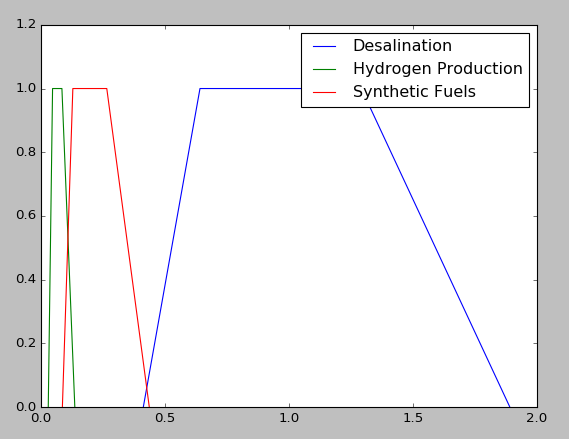
\includegraphics[width=0.5\textwidth]{membership.png}
  \caption{ \small \sl A figure displaying the fuzzy utility function for the three industrial processes.  The furthest to the right has the highest importance. Clearly Desalination has the greatest fuzzy number.}
  \label{memfunc}
\end{figure}


\begin{table}[h!]
\centering
\caption{AHP Survey answers for determining the relative importance of different criteria}
\label{AHPAnswers}
\begin{tabular}{|l|l|l|l|l|l|}
\hline
\begin{tabular}[c]{@{}l@{}}Pairwise \\ Criteria\end{tabular}                       & 1st Expert       & 2nd Expert       & 3rd Expert & 4th Expert       & 5th Expert       \\ \hline
\begin{tabular}[c]{@{}l@{}}Safety vs \\ Flexibility \end{tabular}       & Safety: 6        & Safety: 9        & Safety: 8  & Safety: 6        & Safety: 7        \\ \hline
\begin{tabular}[c]{@{}l@{}}Safety vs \\ Profitability\end{tabular}                 & Safety: 8        & Safety: 8        & Safety: 8  & Equal            & Safety: 7        \\ \hline
\begin{tabular}[c]{@{}l@{}}Ability to \\ Fluctuate\\ vs Profitability\end{tabular} & Profitability: 8 & Profitability: 7 & Equal      & Profitability: 8 & Profitability: 4 \\ \hline
\end{tabular}
\end{table}

\newpage
\section{AHP Conclusion and Future Work}

AHP should be used early in the design and decision making process to determine the best options given a set of criteria. Unlike other systems which can be compared to experimental setups, AHP evaluates systems which cannot have large scale experiments. Given the criteria of safety, flexibility, and profitability a multi-stage flash distillation system appears to be the best choice in a generic setup when compared with synthetic fuels upgrading and hydrogen production from high temperature steam electrolysis. In future work applying AHP to \ac{nrhes} configurations, considerations such as access to feedstocks, for example water and hydrocarbons, will likely play a large role in determining the industrial process incorporated.

 Future work on applying AHP to \ac{nrhess} would include many more criteria, subcriteria, and alternatives which are important to evaluate on a relative basis.  Criteria such as emissions, a key driver for \ac{nrhess}, would be important to consider before determining the optimal industrial process for a given industrial park. Other criteria such as likely regulatory barriers and state of development of the industrial process technology would also be valuable to include in future research.
